------------------------------------------------------------------------

\documentclass{fancyslides}

\usepackage[utf8]{inputenc} % Allows the usage of non-english characters
\usepackage{times} % Use the Times font
\usepackage{booktabs} % Allows the use of \toprule, \midrule and \bottomrule in tables
\graphicspath{{images/}} % Location of the slide background and figure files

% Beamer options - do not change
\usetheme{default} 
\setbeamertemplate{navigation symbols}{} % Disable the slide navigation buttons on the bottom of each slide
\setbeamercolor{structure}{fg=\yourowntexcol} % Define the color of titles and fixed text elements (e.g. bullet points)
\setbeamercolor{normal text}{fg=\yourowntexcol} % Define the color of text in the presentation

%------------------------------------------------
% COLORS
% The following colors are predefined in this class: white, black, gray, blue, green and orange

% Define your own color as follows:
%\definecolor{pink}{rgb}{156,0,151}

\newcommand{\structureopacity}{0.75} % Opacity (transparency) for the structure elements (boxes and circles)

\newcommand{\strcolor}{blue} % Set the color of structure elements (boxes and circles)
\newcommand{\yourowntexcol}{white} % Set the text color

%----------------------------------------------------------------------------------------
%	TITLE SLIDE
%----------------------------------------------------------------------------------------

\newcommand{\titlephrase}{LES SYSTEMES DE CLASSIFICATION D'IMAGES} % Presentation title
\newcommand{\name}{kamelia admanta et agbodjan edoe junior} % Presenter's name
\newcommand{\affil}{PPEI} % Presenter's institution

\begin{document}

\startingslide % This command inserts the title slide as the first slide

%----------------------------------------------------------------------------------------
%	PRESENTATION SLIDES
%----------------------------------------------------------------------------------------

\fbckg{4.png} % Slide background image 
\begin{frame}    
\end{frame}
%------------------------------------------------

\fbckg{process.png} % Slide background image
\begin{frame}
\end{frame}

%------------------------------------------------
\fbckg{th.png} % Slide background image
\begin{frame}
\end{frame}

%------------------------------------------------
\fbckg{blank} % A blank background can be used instead of an image
\begin{frame}
\sources{ % An environment for giving credit for slide backgrounds, images will need to be scaled down if there are more than two
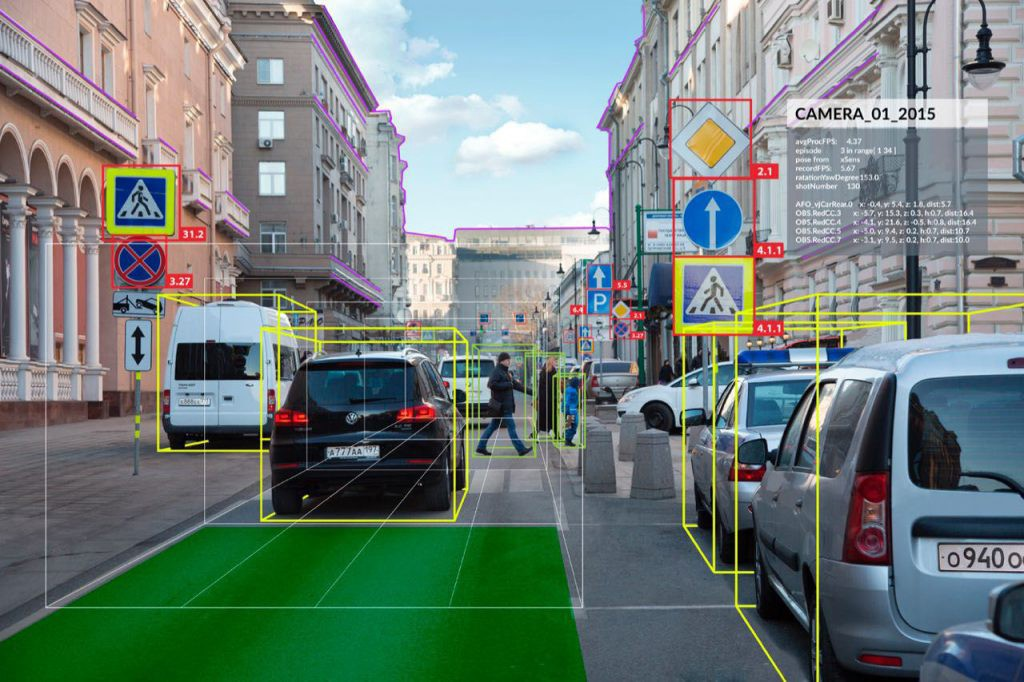
\includegraphics[scale=0.2]{cas1.jpeg} \ voitures autonomes\\
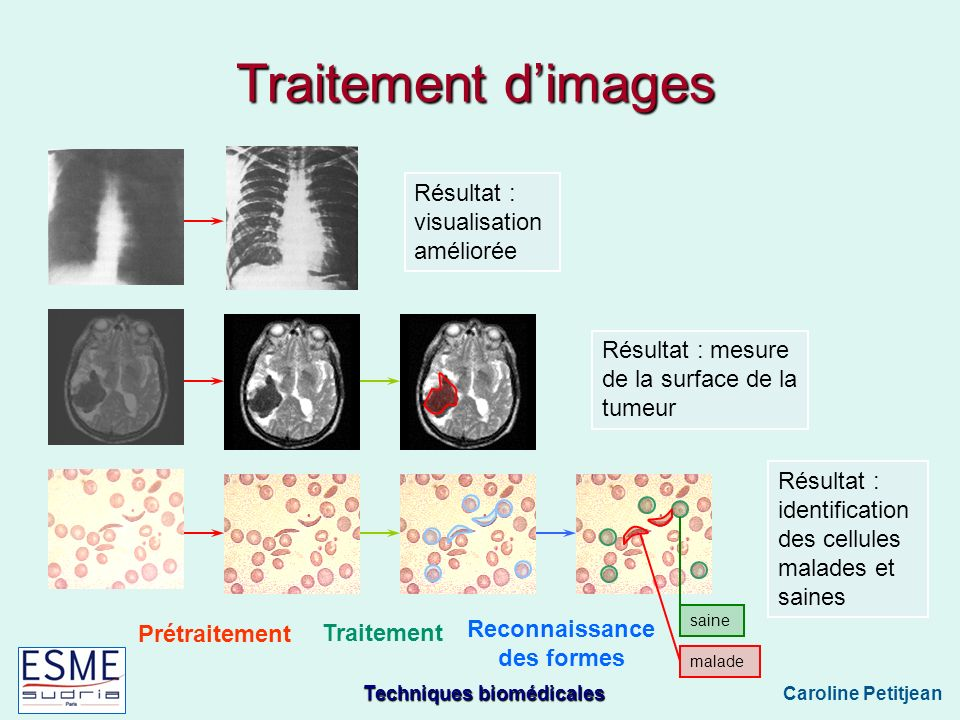
\includegraphics[scale=0.2]{Reconnaissance+des+formes.jpg} \ Medecine
}
\end{frame}
%----------------------------------------------------------------------------------------

\end{document}